\label{research}
So far, we discussed an extension of the pilot abstraction to support data analytics and task based data intensive applications on HPC resources, a comparison between different task-based data oriented frameworks, and a design comparison for executing scientific workflows.
In this section, we motivate and propose a Campaign Manager (CM) to execute scientific campaigns via creating and enacting a campaign execution plan on heterogeneous and dynamic HPC resources. \mtnote{Do we need to explain how these three topics fit together?}\gpnote{I am not sure}

\subsection{Proposed Topic}
Scientific campaigns execute workflows on resources with a given objective~\cite{casajus2010dirac}, often for long periods of time~\cite{maeno2008panda}.
% \mtnote{I think the two are not mutually exclusive: executions of campaigns can have both a given objective and run for a large period of time.}
The objective of a campaign can be translated to a computational objective function that would either minimize or maximize a metric. Among the many metrics that could be considered, the most common one is the total time taken by a campaign to execute. 
Calculating the makespan of the campaign means finding the execution plan that satisfies the computational objective function.


\mtnote{Following the work we did on the separated scratch document, here a brief summary of the 'story' we agreed upon: 
\begin{enumerate}
    \item  General description of the problem space in terms of homo/heterogeneity of campaigns' workflows/resources with the help of the diagram in Figure 1, iterated to show the relevance of space heterogeneity; 
    \item initial formal definition of TTX\_w, including revised list of explicit assumptions, argument about abstraction from resource implementation, list of symbols, and first three equations (r=1, w=\{space/time homo*, space/time hetero*\}; r=n,  w=\{space/time homo*\}; r=n,  w=\{time hetero*\}); 
    \item propose to expand this initial model in the next year by: 
    \begin{enumerate}
        \item relax assumption about homogeneous resources; 
        \item add type heterogeneity of both r and w; 
        \item define m algorithmically; 
        \item if there is time, propose a quantitative definition of m.
    \end{enumerate}
\end{enumerate}}
\gpnote{moved it here}

The way workflows of a given campaign are mapped to resources can affect the makespan calculation. 
Figure~\ref{fig:example_makespan} shows an example of a campaign with workflows of different size and execution times, and the makespans that two different mappings produce.
The makespan of the campaign on the left subfigure is $20$, while on the right it is $16$.
In addition, the size of the workflows, i.e., the number of resources they require, becomes relevant and resources may be underutilized, as shown in Figure~\ref{fig:example_makespan}.

\begin{figure*}[ht!]
    \centering
    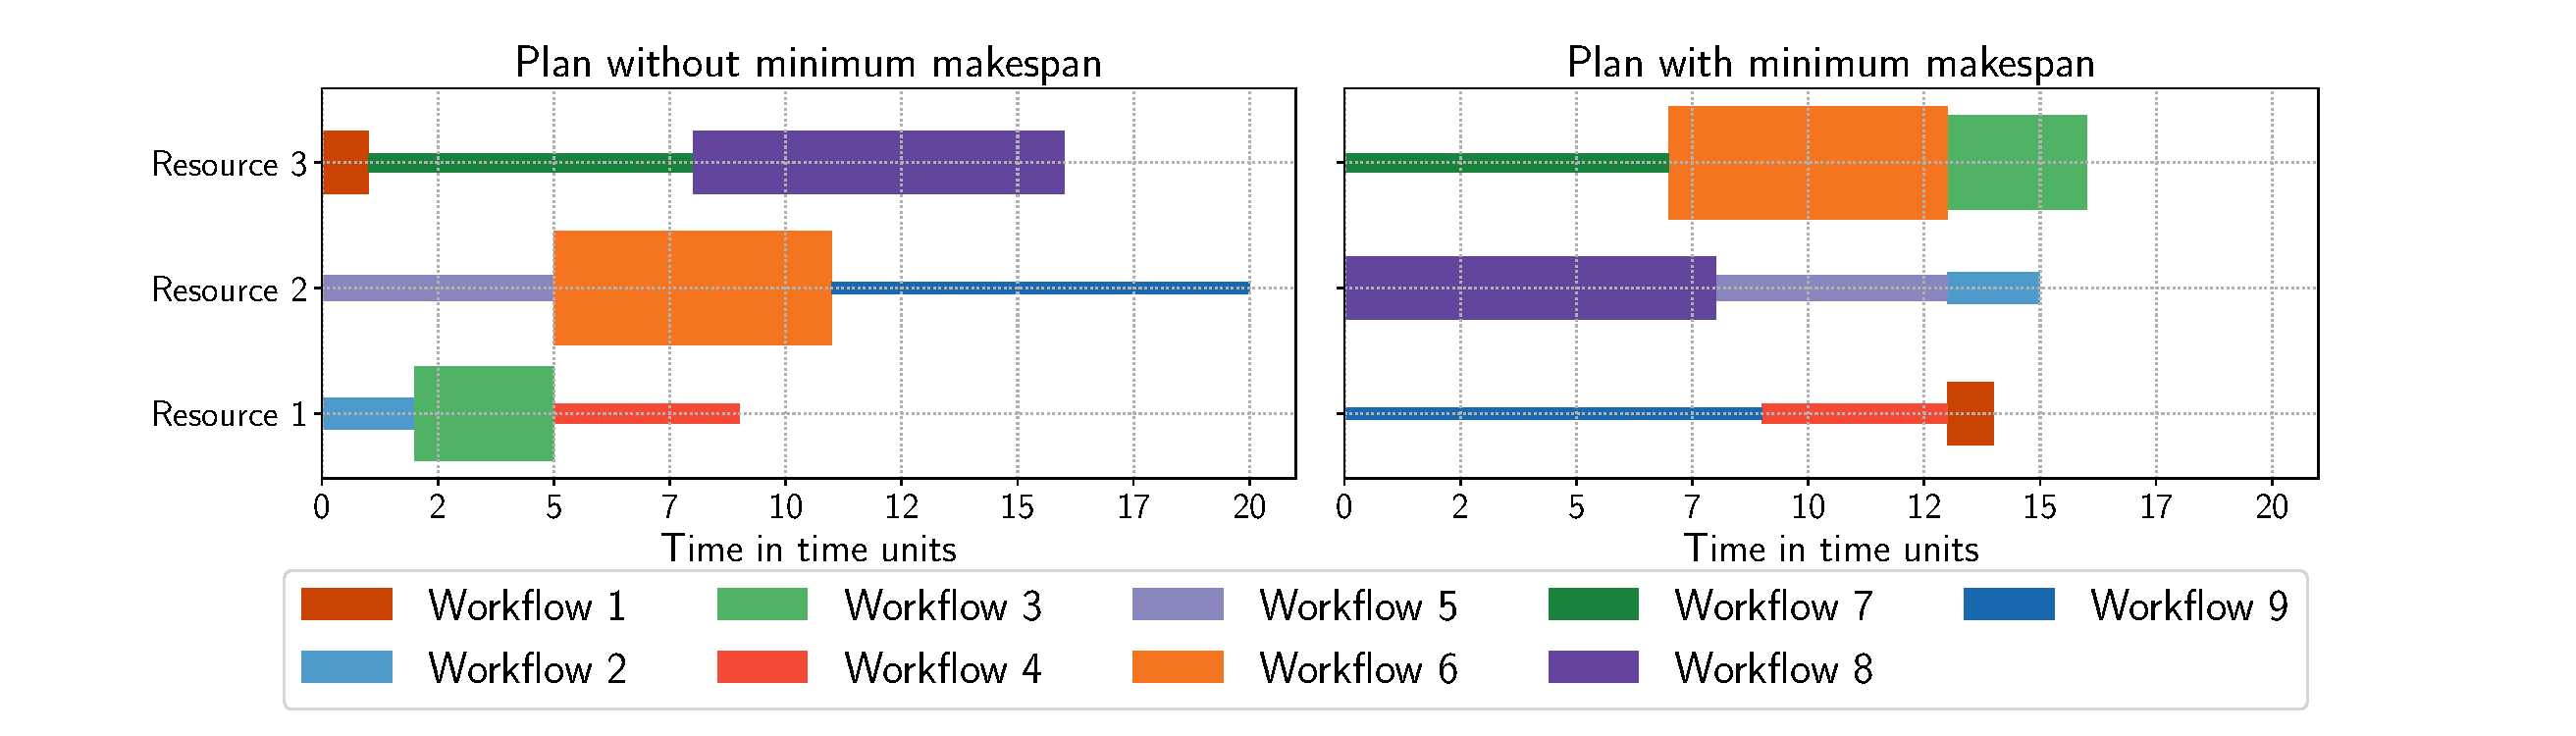
\includegraphics[width=.95\textwidth]{figures/random_vs_specific.pdf}
    \caption{Comparison of different campaign execution plans. Based on workflow mapping on resources makespan and resource utilization is different.}\label{fig:example_makespan}
\end{figure*}

We are making a set of assumptions which we do not relax during the initial analysis of a model that calculates the makespan of a campaign.
These are:
\begin{inparaenum}[(1)]
    \item a workflow is an atomic unit and cannot be decomposed;
    \item workflow resource request is sufficient to execute the workflow; % and the requested resources are utilized;
    \item a resource is an aggregate of computing capabilities;
    \item resources are homogeneous;
    \item every workflow of a given campaign can be executed on the given resources;
    \item a random resource selection is based on a uniform distribution;
    \item only one workflow can be executed on a resource at any point in time; and
    \item a workflows can be homogeneous or heterogeneous in space---maximum number of resources they need, and time---the amount of time they are executing.
\end{inparaenum}

We denote a computational campaign as $C = [w_{i}: 1 \leq i \leq N_{C}]$, where $w_{i}$ is a workflow and $N_{C}$ is the total number of workflows, $R = [ r_{j}: 1 \leq j \leq N_{R}]$ is a set of available resources, where $r_{j}$ is a resource and $N_{R}$ is the total number of available resources, and $ M(C,R) = [(w_i, r_j): 1 \leq i \leq N_{C}, r_j \in R] $ is a mapping function of workflows onto resources.
In addition, we denote the execution time of a workflow as $Tx_{w_{i}}$, the makespan of campaign $C$ as $TTX_{C}$, and the makespan of campaign $C$ for a given mapping function $ M $ as $TTX_{C}(M)$.
Assumption~\#3 allows to abstract the resource implementation details, as workflows can be executed on different resources such as HPCs, Clouds, pilots and more. 
Lastly, we will assume homogeneous resources as it simplifies the formalization of the problem.

With a single resource, i.e., $N_{R} = 1$, the workflows of a campaign will be executed sequentially, regardless the execution order or if the workflows are homogeneous or heterogeneous.
As a result the makespan of the campaign is:
\begin{equation}
   TTX_{C} = \sum_{i=1}^{N_{C}}Tx_{w_{i}} 
\end{equation}

With multiple homogeneous resources, i.e., $1 < N_{R} < N_{C}$, the workflows of a campaign can be executed concurrently.
Furthermore, this is semantically equivalent to executing on a single resource large enough to allow concurrent workflow execution, where each workflow executes on a resource partition. 
Because of assumptions~\#5 and~\#7, executing homogeneous or heterogeneous in space workflows has the same makespan.
A random mapping of workflows onto resource will have a makespan:
\begin{equation}
   TTX_{C}(Random) \geq \frac{1}{N_{R}}\sum_{i=1}^{N_{C}} Tx_{w_{i}} 
\end{equation}
Given multiple homogeneous resources, when executing workflows that are heterogeneous in time and that can be homogeneous or heterogeneous in space, the makespan of the campaign for a given mapping function $ M $ is:
\begin{equation}
TTX_{C}(M) = \max_{r_{j}\in R}\Big\{\sum_{w_{i}\in M(C,r_{j})}Tx_{w_{i}}\Big\}
\label{eq:makespan}
\end{equation}

During the next year, we propose to expand equation~\ref{eq:makespan} by relaxing some of the assumptions we made.
First, we will relax the assumption that resources are homogeneous in terms of (1) maximum number of resources they have available; (2) type of resources, e.g., CPUs or GPGPUs; and (3) the time for which they are available.
Accordingly, we will also assume that workflows may require heterogeneous resources and, as a result, workflows will not be able to be executed on all available resources. 
This will affect the way in which we will have to calculate the makespan of a campaign.
Second, we will introduce resource dynamism to account for how resource availability changes over time. 
This might require to account for dynamic planning, i.e., changing the mapping of workflows to resources based on campaign runtime information.
Third, we will explore algorithmic instances of the mapping function $ M $ such that $TTX_{C}(Random) \geq TTX_{C}(M) \geq min(TTX_{C})$, characterizing and comparing how different algorithmic implementation affect the makespan calculation.
Lastly, if there will be time, we will investigate a quantitative definition of $ M $.

%\mtnote{I think that we will need either equations or diagrammatic representation of the placement + makespan, ideally both. Even knowing quite well what you are trying to write, it is very difficult to follow your argumentation. There are elements of the argumentation (assuming I understand it well enough) that I might disagree with but I am going to keep those thoughts for after the proposal :)}
%\gpnote{separate document moved here.}

% ----------------------------------------------------------------------------
% campaign makespan modeling
We propose to utilize and extend the Heterogeneous Earliest Finish Time (HEFT)~\cite{topcuoglu2002performance} algorithm  as an initial candidate of the function $ M $ for mapping workflows on resources.
%\mtnote{for doing what?}\gpnote{any better?}
HEFT is an offline scheduling algorithm which calculates the makespan of a workflow on heterogeneous resources, in terms of performance.
HEFT has been implemented as part of the planning capabilities in Pegasus~\cite{deelman2015pegasus} and ASKALON~\cite{fahringer2005askalon} amongst other algorithms.
HEFT has been shown to provide better performance in terms of makespan minimization compared to other mapping algorithms~\cite{topcuoglu2002performance,fahringer2005askalon,canon2008comparative}.
This makes HEFT a good candidate for minimizing the makespan of a campaign.
In this context, we propose to evaluate how HEFT performs when compared to a plan in which the mapping between workflows and resources is random.


HEFT makes two important assumptions when used on multiple workflows, i.e., a campaign: (1) any task in a workflow can be executed on all available resources; and (2) all resources are always available.
HEFT is mainly used to derive an execution plan for workflows, i.e., the execution order and resource placement of the tasks that comprise the workflow.
HEFT uses a matrix to represent execution time of tasks on resources, assigning tasks to the resource that minimizes the finish time of the task, and has complexity proportional to the number of dependencies between tasks and the number of resources offered. 
Because we are interested in campaigns, our HEFT extension will provide an execution plan based on workflows as atomic units instead of tasks.
% \mtnote{Why suddenly are we writing about tasks? What is the relationship between HEFT, tasks, workflows and campaigns?}\gpnote{HEFT was created to work on workflows. I added the next paragraph to show how HEFT for campaigns might be different.}
Furthermore, there has been some initial research to extend HEFT to resources that provide CPU and GPUs~\cite{shetti2013optimization}, as well as a HEFT extension on dynamic resources~\cite{dong2007pfas}. 
We will build upon these initial results when investigating how to calculate the makespan of campaigns executed on different types of resources.

We identify three points of possible extensions, so that HEFT is utilized for campaigns.
These are:
\begin{inparaenum}[(i)]
    \item to support heterogeneous workflows;
    \item to support heterogeneous resources; and
    \item to support dynamic resources, as they may become (un)available during execution.
\end{inparaenum}
As a result, HEFT's data structure and algorithm need to be extended to identify whether a workflow can be executed on a given resource, and whether a resource is available.
Finally, a resource may have enough capacity so that multiple workflows can be executed concurrently.
%We will investigate how HEFT can be extended to partition resources  variable resource capacity.\gpnote{It may need further extension.}

There are several alternative methods and algorithms to calculate and optimize the makespan of a workflow~\cite{lu2019review}, including queuing networks~\cite{yao2019throughput,bao2019performance}, domain specific languages~\cite{carothers2017durango,maheshwari2016workflow}, and machine learning~\cite{witt2019predictive,pumma2017runtime}.
Queuing networks will be of limited use because they require from the user to provide a queuing network equivalent to the campaign.
In the case the campaign contains only independent workflows, a single queuing system with multiple servers would be sufficient, but a campaign with complex dependencies between workflows may require expertise outside the user's domain to define the equivalent queuing network.
HEFT sorts workflows based on the number of dependencies they have in the campaign.
Furthermore, using queuing systems to derive the makespan of a campaign requires to search for possible mappings and keep the one that optimizes the makespan, while HEFT uses a heuristic to derive an execution plan.
% \mtnote{These two sentences are unclear, please revise.}\gpnote{any better?}

Domain specific languages approaches either require description of the resource usage of workflows~\cite{carothers2017durango}, or execute part of the campaign to obtain an execution ``skeleton'' of the campaign~\cite{maheshwari2016workflow}.
When executing a campaign, workflows may require days to execute to obtain execution time information, and users rarely know the resource usage of their workflows to provide accurate enough information.
In addition, the workflows of a campaign may be different and executing some of them may not provide any information about the execution of others.
Note that HEFT also requires an initial estimation of the execution time of the workflows, and we plan to utilize initial estimations provided by the user. 
Part of our investigation will be to evaluate how precise this information needs to be in order to obtain an effective plan, i.e., a plan that performs better than a random mapping of campaign workflows on available resources.

%\mtnote{This is unconvincing: we choose to use the PST model and then we say that it requires too much effort? Remember: the argumentation here has to be `scientific', not just based on 'I want to use EnTK so this would require too much time'.}\gpnote{I removed the EnTK argument.}
%Similarly, machine learning approaches would be of limited use since there is no guarantee that the workflows of a campaign is are going to be similar.
%As a result, to gather enough information to build a makespan calculation model may require the execution of the campaign\mtnote{Why would this be a problem?}\gpnote{changed it}.
%We want to provide an approach that only requires the user to provide as few information as possible, such as the workflows and an educated guess of their execution time\gpnote{any better?}.

% ----------------------------------------------------------------------------
% Campaign Manager definition, requirements, features and capabilities
We propose to design a campaign manager (CM) which, given a campaign, an objective, and a set of constraints, can derive an execution plan by utilizing the proposed makespan HEFT algorithm, and execute a campaign.
If necessary the CM will change the execution plan by updating workflow to resource mapping, and resource availability.
Execution planning for workflows are provided by several workflow execution systems, such as Pegasus~\cite{deelman2015pegasus}, and ASKALON~\cite{fahringer2005askalon}.
Campaign management systems, such as PanDA~\cite{maeno2008panda}, do not provide a campaign planning feature.
QCFractal~\cite{qcfractal} offers some form of planning by allowing user to specify the priority of a workflow in a campaign, but this planning does not take into account the makespan of the campaign.

%\mtnote{only these two among all the existing systems? Please refine and expand, explaining that these are just examples. Also, expand appropriately introducing the notions of planning and plan and explaining why they relate to campaign management.}\gpnote{I introduced the plan a few paragraphs before. It may still need to be expanded.}

Currently, campaign managers are making assumptions about the resources and the middleware they are utilizing, are monolithic software systems, and tend to be domain specific.
The CM we propose to prototype will avoid these three limitations. 
Our CM will support multiple use case from different domains, such as molecular dynamics and earth sciences.
As a result, it will be domain agnostic.
In addition, our CM will also be designed by following the building blocks approach~\cite{turilli2019middleware}. 
In this way, it will be agnostic of the system used to manage the execution of the campaign workflows.
This, in turn, will allow our CM to make no assumptions about the resources on which the campaign workflows will be mapped and executed.

Figure~\ref{fig:refarch} shows a reference architecture where the CM has three components:
\begin{inparaenum}[(1)]
\item a Planner;
\item an Enactor; and
\item a Bookkeeper. 
\end{inparaenum}
Workflow execution will be managed by an existing workflow management framework (WMF) on HPC resources.
Plan updates will be based on workflows execution metrics provided by the selected WMF such as tasks execution time, overheads calculation and time to completion.
These metrics will be aggregated across workflows, resulting in campaign-wide execution metrics.

\begin{figure*}[t]
    \centering
    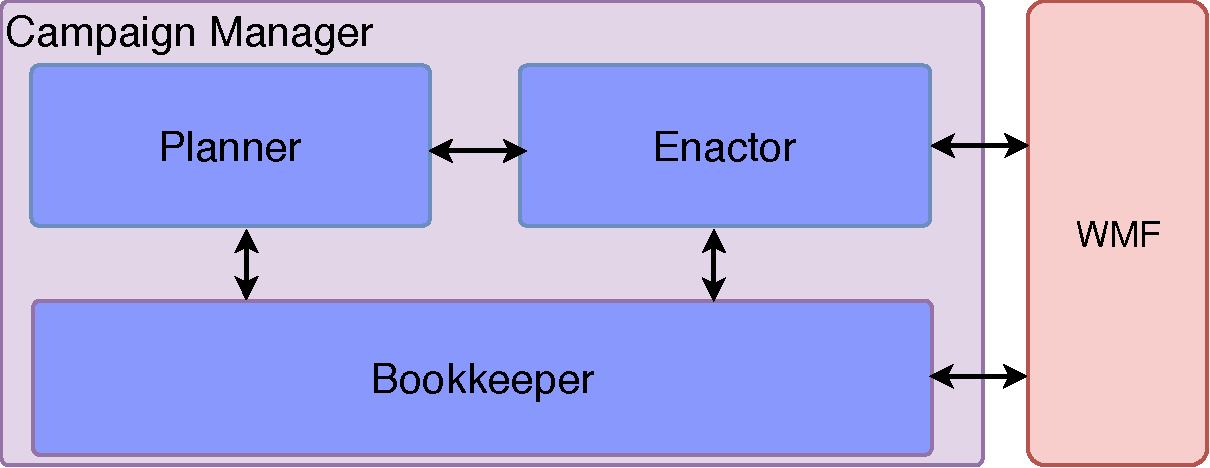
\includegraphics[width=.95\textwidth]{figures/CEM_design.pdf}
    \caption{Reference Architecture of a Campaign Manager. Basic 
    components of Campaign Manager (CM): 1) Planner, 2) Enactor and 3) Bookkeeper. 
    CM communicates decisions to Workflows Management Framework. CM communicates with HPCs to 
    execute parts of the campaign.}\label{fig:refarch}
\end{figure*}

The planner will use the proposed extension of the HEFT algorithm to derive an execution plan, calculating the makespan of a campaign based on the set of available resources and the given objective. 
The planner will pull information about the state of resources as well as the state of the workflows of the campaign from the bookkeeper component.
In addition, based on information from the other components, the planner might be able to update the plan during the campaign runtime. 

%\mtnote{is it a calculator or an optimizer? Seem different capabilities to me and not necessarily part of the same component}\gpnote{any better?}\mtnote{It seems to me that makespan calculation is only one of the elements needed to derive a plan. As such, I think you need at least two components in your architecture: makespan calculator and planner.}\gpnote{The planner uses the makespan calculation to derive a plan. I do not think they should be two different components.}

The Bookkeeper component will be responsible for monitoring the execution of the campaign.
This component will know the state of the campaign, the execution plan, the availability of the resources, and the campaign's objective.
The state of the campaign will be based on information that the bookkeeper will receive from the WMF and the enactor component.
In addition, the bookkeeper will know the state of the resources the campaign is utilizing at runtime and the state of the resources that are planned to be used.
Based on this set of information, the bookkeeper will check whether the campaign's objective can be achieved.
The bookkeeper will inform the planner to update the plan when changes in the campaign happens that affect the effectiveness of a current plan or make the stated objective not achievable. 
For example, workflows could be removed or added to the campaign, or the availability of one or more resources could change requiring a revision of the mapping of workflows to resources or making such mapping impossible.
%An important feature of the bookkeeper will be to identify the reason of a failing workflow.
%When the failure is because the resource is not available, the specific workflow may need to be executed and the plan to be updated.

The enactor will be responsible to execute the planner's plan by interfacing with the WMF.
Based on the plan, the enactor will be responsible to execute workflows on the assigned resources.
To achieve that, the enactor will inform the WMF to acquire resources, translates the workflow from the user's specification to the API provided by the WMF, and submits the workflow for execution.
In the case where a group of workflows is to be executed as a single workflow, the enactor will be responsible to group them as well.
Furthermore, the enactor will inform the bookkeeper about which workflows were submitted for execution.

Scientific workflows are mainly executed by utilizing dedicated workflow management frameworks (WMFs), such as RADICAL-Ensemble Toolkit~\cite{balasubramanian2018harnessing}, Pegasus~\cite{deelman2015pegasus} and others.
These frameworks offer runtime capabilities, such as task execution, data dependency resolution, and workflow definition and monitoring.
Given a set of resources and a walltime, WMFs try to maximize resource utilization and minimize time to completion.
WMFs assume that the user selects sufficient resources and walltime to execute the workflow.
Some WMFs, such as Dask~\cite{rocklin2015dask} and Airflow~\cite{airflow}, provide capabilities to elastically adapt resources, by scaling up or down, based on the current state of execution.
In addition, some  WMFs~\cite{deelman2015pegasus} may also support the concurrent execution of multiple workflows as independent entities, but not a single unified entity to achieve a single objective.

For prototyping our CM, we propose to use the RADICAL-Ensemble Toolkit~\cite{balasubramanian2018harnessing} (EnTK) WMF.
EnTK fits the requirements of the target use cases, and utilizes a pilot framework as runtime system. 
This is fundamental to assure the end-to-end capability required by our prototyping effort when executing real-life use cases. 
Pilots allow to transparently adapt the degree of concurrent and sequential execution of workflow's tasks, supporting our assumption of atomicity at workflow level. 
Further, pilots support the concurrent execution of multiple workflows, depending on the size of the pilot. 
Together, these capabilities guarantee we will be able to investigate makespan calculations for both heterogeneous workflows and resources. 
Finally, since EnTK already supports the execution of the workflows of our target use cases, we will be able to isolate our effort to the prototyping of our CM, offering better chances to complete the proposed activities within the given time frame.

EnTK defines workflows as a set of pipelines, each pipeline is a sequence of stages, and in turn each stage a set of tasks.
Concurrency during execution happens at the level of pipelines and tasks transparently. 
This allows separation of concerns between CM and WMF: CM maps whole workflows to resources while WMF manages the execution of the components of each workflow.
EnTK supports the execution of a sequence of workflows by either reusing already acquired resources or by requesting new ones, enabling the CM to revise its plan based on resource dynamism.
% \mtnote{grammar: from `may' onwards I do not understand the sentence anymore.}\gpnote{fixed it}
EnTK workflow execution is stateful and provides execution timing traces for tasks and workflows, supporting workflow execution on multiple HPC resources. 
This will be of paramount importance to profile and characterize the performance of our CM prototype.
Finally, EnTK utilizes a pilot runtime system, RADICAL-Pilot~\cite{merzky2019using}, to execute workflows on HPC resources.
% Pilot systems submit job placeholders on resources, and are able to execute tasks on the acquired resources.
% This capability allows to execute multiple workflows to resources that are acquired once, either sequentially or concurrently.
The proposed campaign manager will interface with EnTK through the enactor and bookkeeper components to execute and monitor workflows based on the derived execution plan.

\mtnote{General note: this needs to be expanded following the comments I left. At the moment, a lot of this still reads as a set of sometimes disconnected statements. We need to iterate so to produced a more detailed description of the research you propose to conduct in the next year, a description backed by existing literature and your own argumentation. From our discussions, I know you have the material needed to iterate this initial draft.}\gpnote{Let me know how much this comment still holds.}
